\documentclass[11pt,a4paper]{article}
% ukazi za delo s slovenscino -- izberi kodiranje, ki ti ustreza
\usepackage[slovene]{babel}
%\usepackage[cp1250]{inputenc}
\usepackage[T1]{fontenc}
\usepackage[utf8]{inputenc}
\usepackage{amsmath,amssymb,amsfonts,amsthm}
\usepackage{url}
%\usepackage[normalem]{ulem}
\usepackage[dvipsnames,usenames]{color}
\usepackage{graphicx}
\usepackage{enumitem}
\usepackage{tikz}
%\usetikzlibrary{arrows.meta}
%\usetikzlibrary{shapes.geometric}
\usetikzlibrary{positioning}
\usepackage[parfill]{parskip}

% ukazi za matematicna okolja
\theoremstyle{definition} % tekst napisan pokoncno
\newtheorem{definicija}{Definicija}[section]
\newtheorem{primer}[definicija]{Primer}
\newtheorem{opomba}[definicija]{Opomba}

\renewcommand\endprimer{\hfill$\diamondsuit$}

\theoremstyle{plain} % tekst napisan posevno
\newtheorem{lema}[definicija]{Lema}
\newtheorem{izrek}[definicija]{Izrek}
\newtheorem{trditev}[definicija]{Trditev}
\newtheorem{posledica}[definicija]{Posledica}


% za stevilske mnozice uporabi naslednje simbole
\newcommand{\R}{\mathbb R}
\newcommand{\N}{\mathbb N}
\newcommand{\Z}{\mathbb Z}
\newcommand{\C}{\mathbb C}
\newcommand{\Q}{\mathbb Q}

% ukaz za slovarsko geslo
\newlength{\odstavek}
\setlength{\odstavek}{\parindent}
\newcommand{\geslo}[2]{\noindent\textbf{#1}\hspace*{3mm}\hangindent=\parindent\hangafter=1 #2}

% naslednje ukaze ustrezno popravi
\newcommand{\program}{Matematika} % ime studijskega programa: Matematika/Finan"cna matematika
\newcommand{\imeavtorja}{Ines Meršak} % ime avtorja
\newcommand{\imementorja}{prof.~dr. Sandi Klavžar} % akademski naziv in ime mentorja
\newcommand{\naslovdela}{Problem londonskega stolpa}
\newcommand{\letnica}{2016} %letnica diplome


% commands
\newcommand{\graf}[1][G]{\ensuremath{#1 = (V(#1), E(#1))}}
\newcommand{\vozlisca}[1][G]{\ensuremath{V(#1)}}
\newcommand{\povezave}[1][G]{\ensuremath{E(#1)}}
\newcommand{\bd}{\ensuremath{|\,}}
\newcommand{\ed}{\ensuremath{\,|}}
% operatorji
\DeclareMathOperator {\stopnja} {deg}

\title{Problem londonskega stolpa}
\author{Ines Meršak}
\date{13.~05.~2016}


\begin{document}

\maketitle

 
% tu se zacne tekst seminarja
\section{Klasični problem londonskega stolpa}

\begin{itemize}
    \item izumil Tim Shallice, profesor nevropsihologije, leta 1982
    \item pogosto je uporabljen predvsem na področju nevropsihologije, in sicer za opazovanje sposobnosti načrtovanja ter ugotavljanje napredka nekaterih bolezni
    \item tri enako velike krogle različnih barv
    \item tri palice različnih velikosti
    \item na prvo palico lahko postavimo samo eno kroglo, na drugo le dve krogli, na tretjo pa tri
    \item cilj igre je priti iz nekega danega stanja v neko drugo želeno stanje z minimalnim številom potez
\end{itemize}

Označimo krogle s številkami 1, 2, 3, pri čemer je npr.\ krogla 1 modra, krogla 2 rdeča, krogla 3 pa rumena. Začetek naslednje palice bomo nakazali s $|$, krogle pa bomo naštevali od vrha proti dnu palice.
Na primer: stanja na prejšnji sliki so $|3|12$ in $|21|3$.

%\subsection{Osnovne definicije teorije grafov}
%
%\begin{itemize}
%    \item graf je \emph{povezan}, če za poljuben par vozlišč obstaja sprehod med njima
%    \item \emph{premer} grafa je največjo minimalna razdalja med pari vozlišč; če vzamemo poljubno vozlišče v grafu, potem lahko pridemo do drugega poljubnega vozlišča preko $d$ ali manj povezav, kjer je $d$ premer grafa
%    \item graf je \emph{ravninski}, če ga lahko narišemo v ravnini tako, da se nobeni povezavi ne križata
%\end{itemize}

\subsection{Graf klasičnega problema londonskega stolpa}
S pomočjo teh oznak lahko opišemo vsako možno stanje in narišemo graf londonskega stolpa, pri čemer so vozlišča stanja, povezave pa so med tistimi stanji, med katerimi lahko prehajamo z eno potezo (enim veljavnim premikom krogle).

%\begin{figure}[h]
%    \centering
%    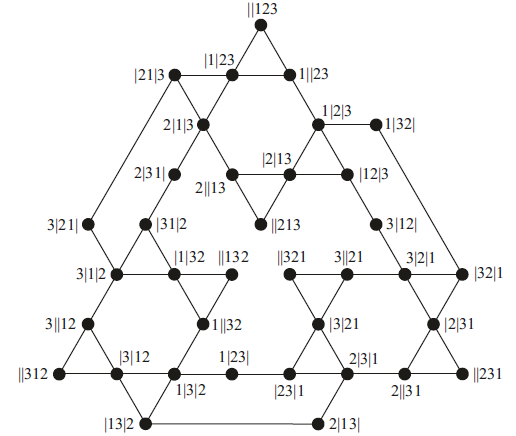
\includegraphics[height=200pt]{../img/tolgraph.png}
%\end{figure}

%\begin{lema}
%    \label{lem:stanja-klas-lond}
%    Število vseh možnih stanj klasičnega londonskega stolpa je 36.
%\end{lema}

\begin{itemize}
    \item 36 vozlišč (lahko preštejemo)
    \item po 12 vozlišč stopnje 2, 3, 4
    \item premer grafa je 8
    \item ravninski (narisan je v ravnini, povezave se nikjer ne križajo)
\end{itemize}

\medskip

\begin{trditev}
    Graf $L$ vsebuje Hamiltonovo pot, ne pa tudi Hamiltonovega cikla.
\end{trditev}

\begin{proof}[Oris dokaza]
    Hitro lahko dokažemo, da $L$ vsebuje Hamiltonovo pot: poiščemo jo. Ena izmed Hamiltonovih poti v grafu $L$ je prikazana na sliki.
    
    Da bi dokazali, da graf ni Hamiltonov, najprej opazimo nekaj lastnosti tega grafa, potem pa poskušamo konstruirati tak cikel v grafu, ki bi šel skozi vsa vozlišča natanko enkrat, a vidimo, da takega cikla ne moremo konstruirati.
    
%    Soseščina vsakega vozlišča stopnje 2 je sestavljena iz enega vozlišča stopnje 3 in enega stopnje 4, prav tako je presek soseščin poljubnih dveh vozlišč stopnje 2 prazen -- vsako vozlišče stopnje 2 ima torej ``svoje'' vozlišče stopnje 3 in stopnje 4. Nadalje lahko iz grafa vidimo, da poljubni dve vozlišči stopnje 3 nista sosednji.
%    
%    Sledi, da na ciklu $C$ v grafu, ki bi vseboval vsa vozlišča, nobeni dve vozlišči stopnje 4 nista sosednji. Ker imamo po 12 vozlišč vsake stopnje, bi v nasprotnem primeru namreč prišli do zaključka, da morata biti sosednji dve vozlišči stopnje 3, kar pa je v protislovju z zgornjim opažanjem.
\end{proof}

\section{Posplošeni londonski stolp}
Graf klasičnega problema je majhen, možnih stanj je malo, zato je za testiranje odraslih ljudi naloga včasih prelahka; Jenny R.\ Tunstall je prva predlagala razširitev na 4 krogle s podaljšanimi palicami (vsaka je podaljšana za eno enoto).

\subsection{Definicija}

Poglejmo si posplošitev tega problema na $p$ palic in $n$ krogel različne barve, pri čemer je $p \geq 3 \text{ in } n \geq 2$. Vsako palico označimo s številom $k \in [p]$, pri čemer je $h_k$ višina palice (ta predstavlja število krogel, ki jih drži palica). Krogle označimo z 1 do $n$ -- te lahko razporejamo na palice. Veljati mora $n \leq \sum_{k=1}^p h_k$, torej da lahko vse krogle razporedimo na palice. 
Poteza je veljavna, če vrhnjo kroglo neke palice prestavimo na vrh druge, pod pogojem, da je na tej palici manj kot $h_k$ krogel.

Vsako stanje krogel lahko enolično predstavimo s permutacijo $s \in S_{n+p}$, $S$ je simetrijska grupa. Pri tem je $s_i$ položaj krogle $i$, če $i \in [n] $, ali dna palice $i-n$, če je $i \in [n+p] \setminus [n] $. Položaje oštevilčimo od leve palice proti desni, z vrha palice proti dnu (kot pri klasičnem problemu). Tako bo s številko 1 oštevilčen položaj krogle, ki je postavljena najvišje na prvi palici; če na prvi palici ni nobene krogle, bo imelo položaj 1 dno te palice.

Naš primer: $s = 452136$.
%{\small $s$ bomo zapisali v obliki $ \sum_1 | \ldots | \sum_p $, kjer je $\sum_k$ niz oznak krogel v položajih od $s_{n+k-1} + 1$ do $s_{n+k}-1$ od vrha palice navzdol. $s_{n+0} = 0$ in ne $s_n$. Vertikalne pipe spet označujejo začetek dna palice.}

\begin{definicija}
    \emph{Londonski graf} $L_h^n$, kjer je $p \geq 3,\ n \geq 2,\ h \in [n]^p,\  \sum_{k=1}^p h_k \geq n$:
    \begin{itemize}
        \item vozlišča: vse permutacije $s \in S_{n+p}$, za katere velja:
        \[\forall k \in [p]:\ 1 \leq s_{n+k} - s_{n+k-1} \leq h_k + 1,\ s_{n+p} = n + p ,\]
        \item povezave: vsaki dve stanji (oz.\ pripadajoči permutaciji), med katerima lahko prehajamo z veljavno potezo, sta povezani
    \end{itemize}
\end{definicija}

Hitro vidimo, da mora veljati 
\[\forall k \in [p]\colon s_{n+k} - s_{n+k-1} \geq 1 \]
saj je $s_{n+k}$ položaj dna palice $k$, $s_{n+k-1}$ pa položaj dna palice $k-1$, torej se mora njun položaj razlikovati najmanj za 1 -- to se zgodi, če na palici $k$ ni nobene krogle.

Prav tako pa mora veljati tudi 
\[\forall k \in [p]\colon s_{n+k} - s_{n+k-1} \leq h_k + 1,\]
kar se zgodi v primeru, če je na $k$-ti palici $h_k$ krogel.

S pogojem, da so vse palice visoke največ $n$, ne izgubimo splošnosti, saj razporejamo le $n$ krogel.

Če smo v primeru klasičnega londonskega stolpa lahko izračunali število vozlišč, pa je v splošnem za londonske stolpe to precej težko. 

\section{Oxfordski graf}

\emph{Oxfordski graf} je poseben primer londonskega grafa, za katerega velja, da so vse palice velikosti $n$, pri čemer je $n$ število krogel. Oxfordski graf označimo z $O^n_p$, zanj torej velja $O^n_p := L^n_{n^p}$.

Medtem ko je v splošnem težko določiti število vozlišč londonskega grafa, pa je to precej bolj preprosto za oxfordski graf. Še več, določimo lahko tudi število povezav.

\begin{trditev}
    Število vozlišč oxfordskega grafa $O^n_p$ je enako \[\frac{(n+p-1)!}{(p-1)!}.\]
\end{trditev}

\begin{proof}[Oris dokaza]
    Iščemo število vseh možnih stanj pri oxfordskemu stolpu. Najprej pozabimo na različne barve krogel. Predstavljamo si, da imamo vse krogle zložene v vrsto, nato pa na poljubna mesta (s ponavljanjem) vrivamo $|$ ; mesta so poljubna, saj so vse palice dovolj visoke, da lahko na njih zložimo vse krogle. Ko vrinemo $p-1$ pip, smo določili $p$ palic in s tem razporeditev krogel. Nato samo še premešamo barve in dobimo končen rezultat.\\
    (neurejeni izbori s ponavljanjem, izbiramo mesta za pipe)
\end{proof}

\begin{trditev}
    Število povezav oxfordskega grafa $O^n_p$ je enako
    \[ \frac{np}{2} \frac{(p-2+n)!}{(p-2)!} .\]
\end{trditev}

\begin{proof}[Oris dokaza]
    Ugotovimo, da so vsa stanja, ki imajo točno $q$ nepraznih palic, $1 \leq q \leq p$ in $n \geq q$, enake stopnje. Preštejemo vsa taka stanja, nakar uporabimo lemo o rokovanju, stopnje vozlišč seštejemo po $q$.
\end{proof}

\begin{lema}[Lema o rokovanju]
    \label{lema:rokovanje}
    Za vsak graf \graf velja formula
    \begin{equation}
    \sum_{u \in V(G)}\! \stopnja u = 2 \cdot |E(G)|.
    \label{eq:lema-o-rokovanju}
    \end{equation}
\end{lema}

\section{Lastnosti londonskega grafa}

\subsection{Povezanost}
Zaželjeno je, da lahko pri londonskem stolpu prehajamo med poljubnima dvema stanjema, saj se problem uporablja za psihološka testiranja. To velja, če je pripadajoči londonski graf povezan, kar je zato ena pomembnejših lastnosti tega grafa.

V nadaljevanju bomo privzeli, da so palice urejene po velikosti naraščajoče, velja torej $h_1 \leq h_2 \leq \cdots \leq h_p$.
Potreben pogoj za povezanost londonskega grafa je očitno 
\[ n \leq \sum_{k=1}^{p-1} h_k, \]
oziroma z besedami, da lahko krogle razporedimo tako, da najvišja palica ostane prazna. V nasprotnem primeru bi, po tem ko bi razporedili maksimalno možno število krogel na vse preostale (manjše) palice, na največji ostalo še nekaj krogel, ki jih nikoli ne bi mogli premakniti na kakšno drugo palico.
Izkaže se, da je ta pogoj tudi zadosten za povezanost londonskega grafa.

\begin{izrek}
    Londonski graf $L_h^n$ je povezan natanko tedaj, ko velja pogoj
    \begin{equation}
        n \leq \sum_{k=1}^{p-1} h_k.
        \label{eq:pogoj-povezanosti}
    \end{equation}
\end{izrek}

\begin{proof}[Oris dokaza]
    Želimo dokazati, da lahko najdemo pot med poljubnima dvema vozliščema v londonskem grafu, oziroma da lahko prehajamo med poljubnima dvema stanjema krogel. Dokaza se lotimo tako, da problem zreduciramo na vprašanje, ali lahko zamenjamo poljubni dve krogli, brez da bi pri tem spremenili položaj katerekoli krogle, nato pa pokažemo, da je to mogoče.
\end{proof}

\subsection{Ravninskost}

Omenili smo že, da se problem londonskega stolpa pogosto uporablja kot psihološki test. Psihologi rezultate testov radi prikažejo kar na grafu uporabljenega problema, zato je zanimivo tudi vprašanje ravninskosti londonskih grafov -- križanje povezav namreč lahko vodi do zmede pri prikazu rezultatov. Ker se za testiranje uporablja le londonski stolp s tremi palicami, se bomo tudi pri obravnavi ravninskosti omejili na ta primer, torej naj bo $p=3$.

Najprej si poglejmo problem za dve krogli ($n=2$): vsi grafi so ravninski, kot je prikazano na sliki.

Preden si ogledamo problem za $n=3$, se spomnimo operacije \emph{subdivizije}: vzamemo neko povezavo $e$ grafa in na sredino te povezave dodamo še eno vozlišče. Ta operacija ohranja ravninskost.   
%    \item graf $H$ je \emph{subdivizija} grafa $G$, če ga lahko dobimo iz $G$ z zaporednim \emph{subdiviziranjem} povezav grafa $G$; očitno je tak $H$ ravninski natanko tedaj, ko je $G$ ravninski
%    \item hitro lahko vidimo, da grafa $K_5$ in $K_{3,3}$ nista ravninska (poskusimo ju narisati v ravnini, a kmalu ugotovimo, da to ne bo mogoče)
Graf torej zagotovo ni ravninski, če vsebuje subdivizijo $K_5$ ali $K_{3,3}$ (ta dva grafa nista ravninska); zanimivo pa je, da velja tudi obratno.

\medskip

\begin{izrek}[Kuratowski]
    Graf $G$ je ravninski natanko tedaj, ko ne vsebuje subdivizije $K_5$ niti subdivizije $K_{3,3}$.
\end{izrek}

\medskip

\begin{trditev}
    Naj bo $p=3$. Tedaj so londonski grafi $L_h^2, L_{122}^3,L_{123}^3$ in $ L_{133}^3$ ravninski.
\end{trditev}
\begin{proof}[Oris dokaza]
    Za $n=3$ dobimo sledečo shemo:
    
    \[
    \begin{matrix}
    & & L & & & & \\
    & & \parallel & & & & \\
    L_{122}^3 & \subset & L_{123}^3 & \subset & L_{133}^3 & & \\
    \cap & & \cap & & \cap & & \\
    L_{222}^3 & \subset & L_{223}^3 & \subset & L_{233}^3 & \subset & L_{333}^3 \\
    & & & & & & \parallel \\
    & & & & & & O^3_3 \\
    \end{matrix}
    \]
    
    Dokazati moramo še, da londonski grafi za $n \geq 4$ niso ravninski. Pri tem upoštevamo, da nekateri grafi z $n = 4$ vsebujejo nekatere neravninske grafe, v nekaterih moramo pa ponovno poiskati subdivizijo $K_{3,3}$. S tem ugotovimo, da noben londonski graf za $n=4$ ni ravninski, zato niso ravninski tudi grafi za $n>4$.
\end{proof}

% seznam uporabljene literature
\begin{thebibliography}{99}

\bibitem{bib:tohmyths} A. M. Hinz, S. Klavžar, U. Milutinović in C. Petr, \emph{The Tower of Hanoi – Myths and Maths}, Birkhäuser, Basel, 2013.

\bibitem{bib:potocnik} P. Potočnik, \emph{Zapiski predavanj iz Diskretne Matematike I}, 1.~izdaja, [ogled 29.~12.~15], dostopno na \url{http://www.fmf.uni-lj.si/~potocnik/Ucbeniki/DM-Zapiski2010.pdf}

\bibitem{bib:wikishal} \emph{Tim Shallice}, v: Wikipedia: The Free Encyclopedia, [ogled 8.~10.~2015], dostopno na\\ \url{https://en.wikipedia.org/wiki/Tim_Shallice}.

\bibitem{bib:wikihamilpath} \emph{Hamiltonian path}, v: Wikipedia: The Free Encyclopedia, [ogled 28.~12.~2015], dostopno na \url{https://en.wikipedia.org/wiki/Hamiltonian_path}.
\end{thebibliography}

\end{document}

